In this section, we will show how a static table with null entries can be compressed such that almost no null entries must be stored.
The method works only for the static case, which means that all data is added to the table before any of it is looked up.
All tables are basically two-dimensional arrays that have the same number of rows and columns, i.e.\ they are square.
The remaining setup is similar to tries:
We store $n$ integers in the range $0$ through $N - 1$ in the tables.
Since all integers in the range must fit in a table, $N$ is the table size.
The tables are square, so $N$ must be a square and there is an $m$ such that $N = m^2$.
$m$ is then the number of rows and columns.
Further we assume that $n \geq \max(2, m)$.
The cell $(i, j)$ for an integer $k$ can be found by counting rowwise from the top left until $k$ or by the following formula: $i = \l\lfloor \frac{k}{m} \r\rfloor + 1$ and $j = k \operatorname{mod} m + 1$.
The table entry for $k$ contains the information belonging to $k$ if $k$ is present in the table and null otherwise.

\begin{wrapfigure}{r}{0.5\textwidth}
  %\begin{tikzpicture}[align=center, node distance=2cm]
%\matrix (all) [table, text width=7mm]
%{
%	0 & 0 & * & 0 \\
%	* & * & * & 0 \\
%	0 & * & * & 0 \\
%	* & 0 & 0 & * \\
%};

%\matrix (r2) [table, text width=7mm, below of=all]
%	{ * & * & * & 0 \\};
%	
%\matrix (r3) [table, text width=7mm, below of=r2-1-3]
%	{ 0 & * & * & 0 \\};
%	
%\matrix (r4) [table, text width=7mm, below of=r3-1-4]
%	{ * & 0 & 0 & * \\};
%	
%\matrix (r1) [table, text width=7mm, below of=r4-1-3]
%	{ 0 & 0 & * & 0 \\};


\matrix (mx) [%
		matrix of nodes,
		draw = none,
		row sep = 0.7em,
		column sep = 0em
]
{
	$\s$ & $\s$ & $\s$ & 0    & {}   & {}   & {}   & {} & {}   &[1em] $r_2 = 0$ \\
	{}   & {}   & 0    & $\s$ & $\s$ & 0    & {}   & {} & {}   & $r_3 = 2$ \\
	{}   & {}   & {}   & {}   & {}   & $\s$ & 0    & 0  & $\s$ & $r_4 = 5$ \\
	{}   & {}   & {}   & {}   & 0    & 0    & $\s$ & 0  & {}   & $r_1 = 3$ \\
	5    & 6    & 7    & 10   & 11   & 13   & 3    & 0  & 16   & $\phantom{r_1 = } C$ \\
};


\node[draw, fit = (mx-1-1) (mx-1-4)] (1-fit) {};

\node[draw, fit = (mx-2-3) (mx-2-6)] (2-fit) {};

\node[draw, fit = (mx-3-6) (mx-3-9)] (3-fit) {};

\node[draw, fit = (mx-4-5) (mx-4-8)] (4-fit) {};

\node[draw, fit = (mx-5-1) (mx-5-9)] (C-fit) {};


\end{tikzpicture}
  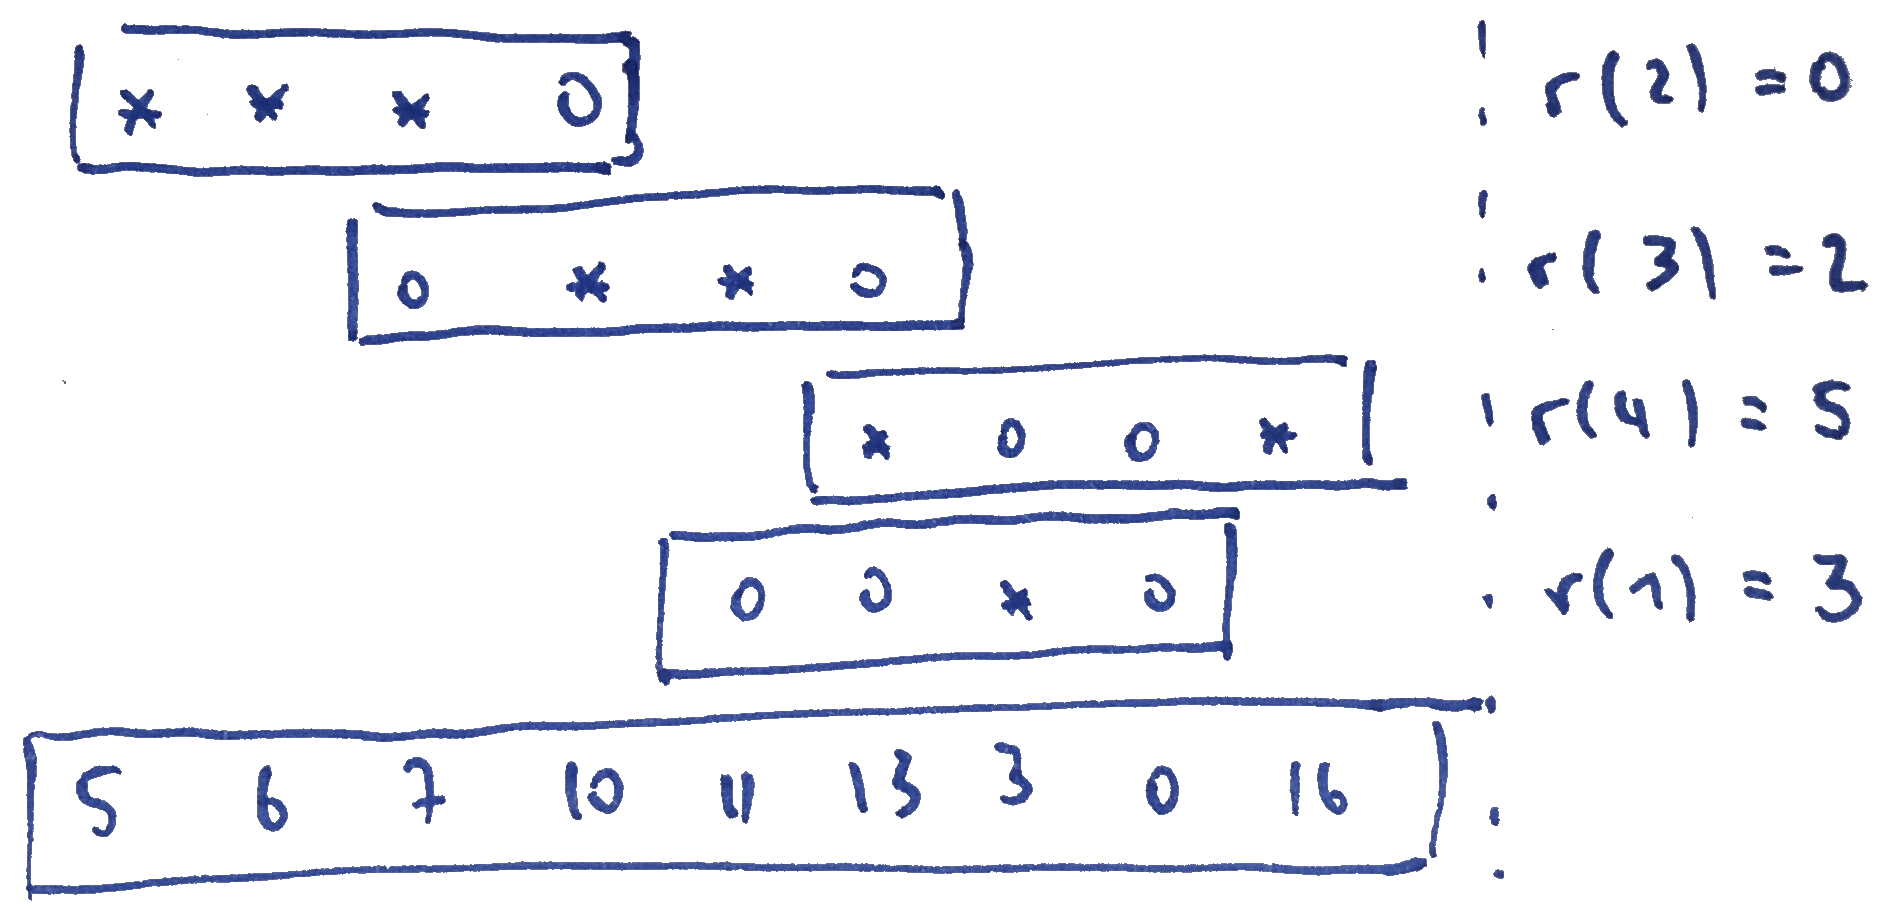
\includegraphics[width=0.5\textwidth]{topic/collapse}
	\caption{Rows of a table collapsed into a one-dimensional array. \label{fig:row_disp}}
\end{wrapfigure}

The compression of such a table $A$ happens in two steps.
Since we consider the static case of table storage, we know all entries before any lookup is performed and we can first insert all $n$ entries into $A$.
Now, we transform $A$ into a one-dimensional array $C$ by mapping every position in $A$ to an index of $C$.
The idea is that we overlap the rows of $A$ so that null entries from previous rows are overwritten by non-null entries of later rows. See Figure~\ref{fig:row_disp}.
Note that the displacement for each row is not calculated in the order in which they appear in the table.
The reason is the following:
Our goal is to minimize the size of $C$.
However, finding the optimal row displacements for a given table is an NP-complete problem.
Instead, we use a heuristic that gives good results for common use cases.
The rows are first sorted by the number of zeroes they contain.
Then we displace every row stepwise until no overlaps with previous rows occur.